\documentclass[]{article}
\usepackage[utf8]{inputenc}
\usepackage{amsthm}
\usepackage{amssymb}
\usepackage{amsmath}
\usepackage{calc}
\usepackage{tikz}
\usepackage{pgfplots}
\begin{document}
\begin{center}
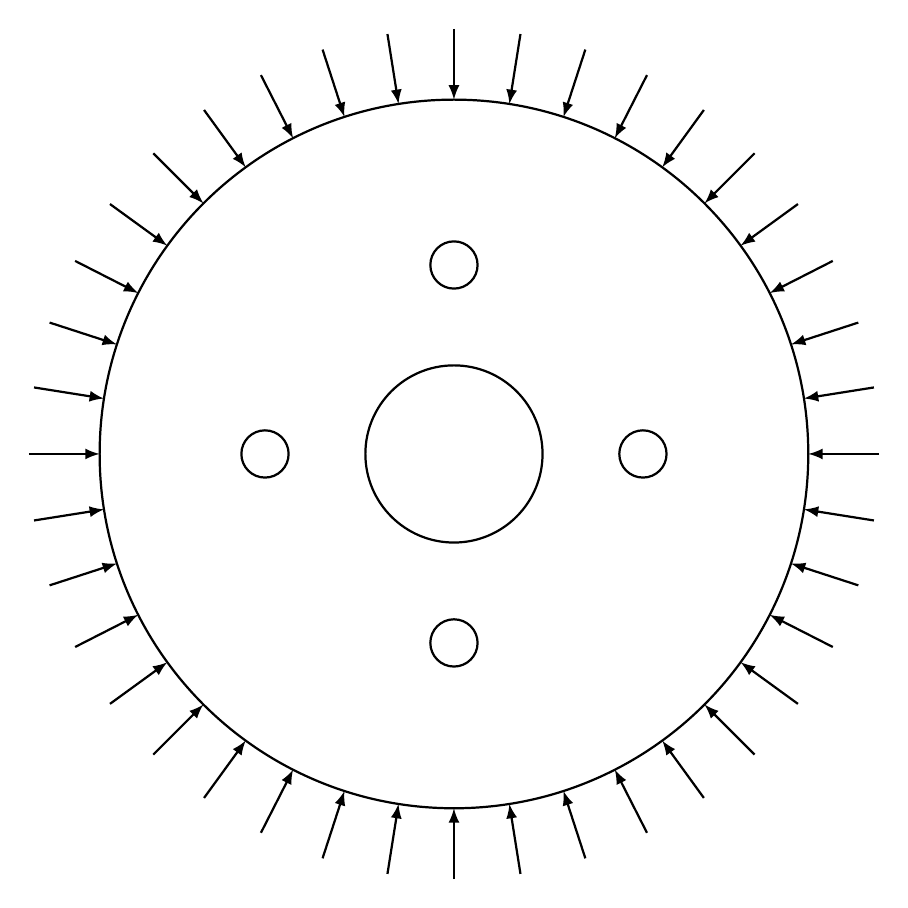
\begin{tikzpicture}[thick]
\def\f{0.015}
\def\ra{\f*300}
\def\raa{\f*360}
\def\ri{\f*75}
\def\rm{\f*160}
\def\d{\f*20}
\def\nC{4}
\def\nA{40}
\draw (0,0) circle (\ra) node {};
\draw (0,0) circle (\ri) node {};
\foreach \x in {1,...,\nC}{
\draw ({\rm*cos(360*\x/\nC)},{\rm*sin(360*\x/\nC)}) circle (\d) node {};}
\foreach \x in {1,...,\nA}{
\draw[>=latex, ->] ({\raa*cos(360*\x/\nA)},{\raa*sin(360*\x/\nA)})--({\ra*cos(360*\x/\nA)},{\ra*sin(360*\x/\nA)});}
\end{tikzpicture}
\end{center}
\begin{align*}
u_r&=C_1r+\frac{C_2}{r}-\frac{1-v^2}{8E}\varrho\omega^2r^3+(1+v)\frac{\alpha}{r}\int_{a}^{r}r'\Delta Tdr'\\
\sigma_r&=\frac{E}{1-v}C_1-\frac{E}{(1+v)r^2}C_2-\frac{3+v}{8}\varrho\omega^2r^2+\frac{E\alpha}{r^2}\int_{a}^{r}r'\Delta Tdr'\\
\sigma_\varphi&=\frac{E}{1-v}C_1+\frac{E}{(1+v)r^2}C_2-\frac{1+3v}{8}\varrho\omega^2r^2+E\alpha(\Delta T-\frac{1}{r^2}\int_{a}^{r}r'\Delta Tdr')
\end{align*}
Aus $\omega=0$ und $\Delta T=0$ folgt:
\begin{align*}
u_r&=C_1r+\frac{C_2}{r}\\
\sigma_r&=\frac{E}{1-v}C_1-\frac{E}{(1+v)r^2}C_2\\
\sigma_\varphi&=\frac{E}{1-v}C_1+\frac{E}{(1+v)r^2}C_2
\end{align*}
Gegeben sind $\sigma_r(r_1)=\sigma_1$ und $u_r(r_2)=0$. Damit kann man $C_1$ und $C_2$  herleiten:
\begin{align*}
0&=C_1r_2+\frac{C_2}{r_2}\\
C_1&=-\frac{C_2}{r^2_2}\tag{1}\\
\sigma_1&=\frac{E}{1-v}C_1-\frac{E}{(1+v)r^2_1}C_2\\
\sigma_1&=-\frac{E}{(1-v)r^2_2}C_2-\frac{E}{(1+v)r^2_1}C_2\\
C_2&=-\frac{\sigma_1(1-v)(1+v)r^2_2r^2_1}{E(1+v)r^2_1+E(1-v)r^2_2}\tag{2}
\end{align*}
Mit $\sigma_1=-100N/mm^2$ und $u_r(r_2)=0\ mm$ folgt:
\begin{align*}
C_1&\approx -3,39\cdot 10^{-4}\\
C_2&\approx 1,90\ mm^2
\end{align*}
\def\CA{-0.000339} %0.0000233
\def\CB{1.90} %3.9
\def\E{200000}
\def\sigR{\E*(\CA/0.7-\CB/(1.3*x*x))}
\def\sigP{\E*(\CA/0.7+\CB/(1.3*x*x))}
\def\sigT{0}
\def\sigV{sqrt(\sigR*\sigR+\sigP*\sigP+\sigT*\sigT-\sigR*\sigP-\sigR*\sigT-\sigP*\sigT)}
\begin{tikzpicture}
\begin{axis}[title=Tangential- und Radialspannung,
xlabel=$r$ in $mm$,
ylabel=$Spannung$ in $N/mm^2$,
grid=major,
domain=75:300,
legend pos=outer north east]
\addplot {\sigR};
\addplot {\sigP};
\legend{$\sigma_r$,$\sigma_\varphi$}
\end{axis}
\end{tikzpicture}\vspace{1cm}\\
Vergleichsspannung
%$$\sigma_v=\sqrt{\sigma_r^2+\sigma_\varphi^2+\sigma_t^2-\sigma_r\sigma_\varphi-\sigma_t\sigma_\varphi-\sigma_r\sigma_t}$$
$$\sigma_v=\sqrt{\sigma_r^2+\sigma_\varphi^2-\sigma_r\sigma_\varphi}$$
\begin{tikzpicture}
\begin{axis}[title=Vergleichsspannung,
xlabel=$r$ in $mm$,
ylabel=$Spannung$ in $N/mm^2$,
grid=major,
domain=75:300,
legend pos=outer north east]
\addplot {\sigV};
\legend{$\sigma_v$}
\end{axis}
\end{tikzpicture}\vspace{1cm}\\
\begin{tikzpicture}
\begin{axis}[title=Verschiebung,
xlabel=$r$ in $mm$,
ylabel=$Verschiebung$ in $mm$,
grid=major,
domain=75:300,
legend pos=outer north east,
scaled y ticks=base 10:2]
\addplot {\CA*x+\CB/x};
\legend{$u_r$}
\end{axis}
\end{tikzpicture}\\
\end{document}
